\documentclass{ieeeaccess}
\usepackage{cite}
\usepackage{amsmath,amssymb,amsfonts}
\usepackage{algorithmic}
\usepackage{graphicx}
\usepackage{textcomp}
\usepackage{pdfpages}




\def\BibTeX{{\rm B\kern-.05em{\sc i\kern-.025em b}\kern-.08em
    T\kern-.1667em\lower.7ex\hbox{E}\kern-.125emX}}
\begin{document}
\history{Date of publication xxxx 00, 0000, date of current version xxxx 00, 0000.}
\doi{10.1109/ACCESS.2017.DOI}

\title{ChoiceMaker: Empowering Sequential Model Optimization with Query Recommendations via Large Language Models}
\author{\uppercase{Feiran Qin}\authorrefmark{1}}
\address[1]{North Carolina State University, Raleigh, NC 27606 USA (e-mail: fqin2@ncsu.edu)}


\tfootnote{
    %This paragraph of the first footnote will contain support 
% information, including sponsor and financial support acknowledgment. For 
% example, ``This work was supported in part by the U.S. Department of 
% Commerce under Grant BS123456.''
}

\markboth
{Author \headeretal: Preparation of Papers for IEEE TRANSACTIONS and JOURNALS}
{Author \headeretal: Preparation of Papers for IEEE TRANSACTIONS and JOURNALS}

\corresp{
    % Corresponding author: First A. Author (e-mail: author@ boulder.nist.gov).
    }

\begin{abstract}
Choice is not only important in human's lifes, but also crucial to software engineering. In CSC 791 Automated Software Engineering class, we are required to implement a Sequential Model Optimizer with Root Mean Square Deviation (RMSE) to the ideal value as the evaluation metric. In this paper, we propose a novel approach that empowers Sequential Model Optimization with Query Recommendations via Large Language Models (LLMs). We first compare RMSE methods with LLMs methods, and then we evaluation the ability of LLMs in different models with different number of tokens, the scalebility of few-shots-learnings, the cost of self-host and commercial models. We find that LLMs [PlaceHolder]. Overall, our approach is able to achieve a better performance than the RMSE methods. 
\end{abstract}

\begin{keywords}
Software Engineering, Large Language Models, Sequential Model Optimization
\end{keywords}

\titlepgskip=-15pt

\maketitle

\section{Introduction}
\label{sec:introduction}
\PARstart{C}{hoice} making is one of the key concerns in software engineering. Long et al.\cite{10352439} argue that, on balance, engineers spend a third of the time in planning, coding, and testing. In software engineering, more than half of the time is allocated to choice-related tasks such as planning, analysis, and testing. Making good choices is important for software reliability. . As the scale of software engineering increases, the data and parameters available become enormous. The number of control parameters of a software package grows linearly with time. Meanwhile, human understanding of those choices only ever grows sub-linearly\cite{10.1145/2786805.2786852}. It's difficult for human beings themselves to make choices that never bad, and bad choice may lead to terrible results. 30\% of all cloud computing errors come from misconfigurations of cloud software\cite{yy}, and even more alarming, 59\% of the most severe performance bugs are caused by poor configuration-- making bad choices one of the most dangerous threats to software quality\cite{10.1145/2961111.2962602}. It turns out that automatically making decisions about choices in software is a great unsung success story. AI tools are very successful at predicting how choices affect software\cite{9734271}.

In CSC 791 Automated Software Engineering \cite{791} classes, Dr. Menzies proposed Sequential Model Optimization with Root Mean Square Deviation (RMSE) to the ideal value as the evaluation metric for decision making, however, RMSE is unaware of the real meaning of data and often mislead by a large single data.

In this work, we propose a novel approach that empowers Sequential Model Optimization with Query Recommendations via Large Language Models(LLMs). The key technical challenges we faced are: 
\begin{itemize}
  

\item \textbf{How to choose the best prompts in balance of accuracy and cost?}
In order to improve the accuracy of LLMs and obtain the desired response, there are several commonly used schemes: zero-shot prompts, few-shot prompts and finetuning. The overhead and benefits of these methods are in increasing order.The cost-effectiveness ratio is determined depends on multiple variables such as the data set, the model, and the optimization objective. We would like to find a quantitative paradigm to guide tunning for datasets of similar sizes.

\item \textbf{How to evaluate the output of LLMs without ground truth?}
Similar to the previous SMO method with RMSE of telling you "how good your options are", the output of LLMs is hard to validate, regardless of whether that’s in the dataset or even feasible. We need to find a way to evaluate the output of LLMs without ground truth. Alternatively, we want to find an experience rule to reverse adjust the prompt to improve the accuracy of LLMs.

\item \textbf{Which model to choose when considering privacy, cost, and accuracy?}
There are various open-source models, such as llama2 , as well as commercial models, such as chatgpt. There are also versions of the open-source model with different token counts, such as 8b, 13b, and 33b. Open-source models are easy to self-host, and are therefore more privacy-friendly, especially when dealing with sensitive or commercial datasets. Commercial models have a performance advantage over open source models, although the gap between them is narrowing. By evaluating the ability of different models on the selection task, we hope to reveal the performance differences between different models, and the evolutionary performance of the ability of models over time.
\end{itemize}

\begin{figure*}[ht]
    \centering
    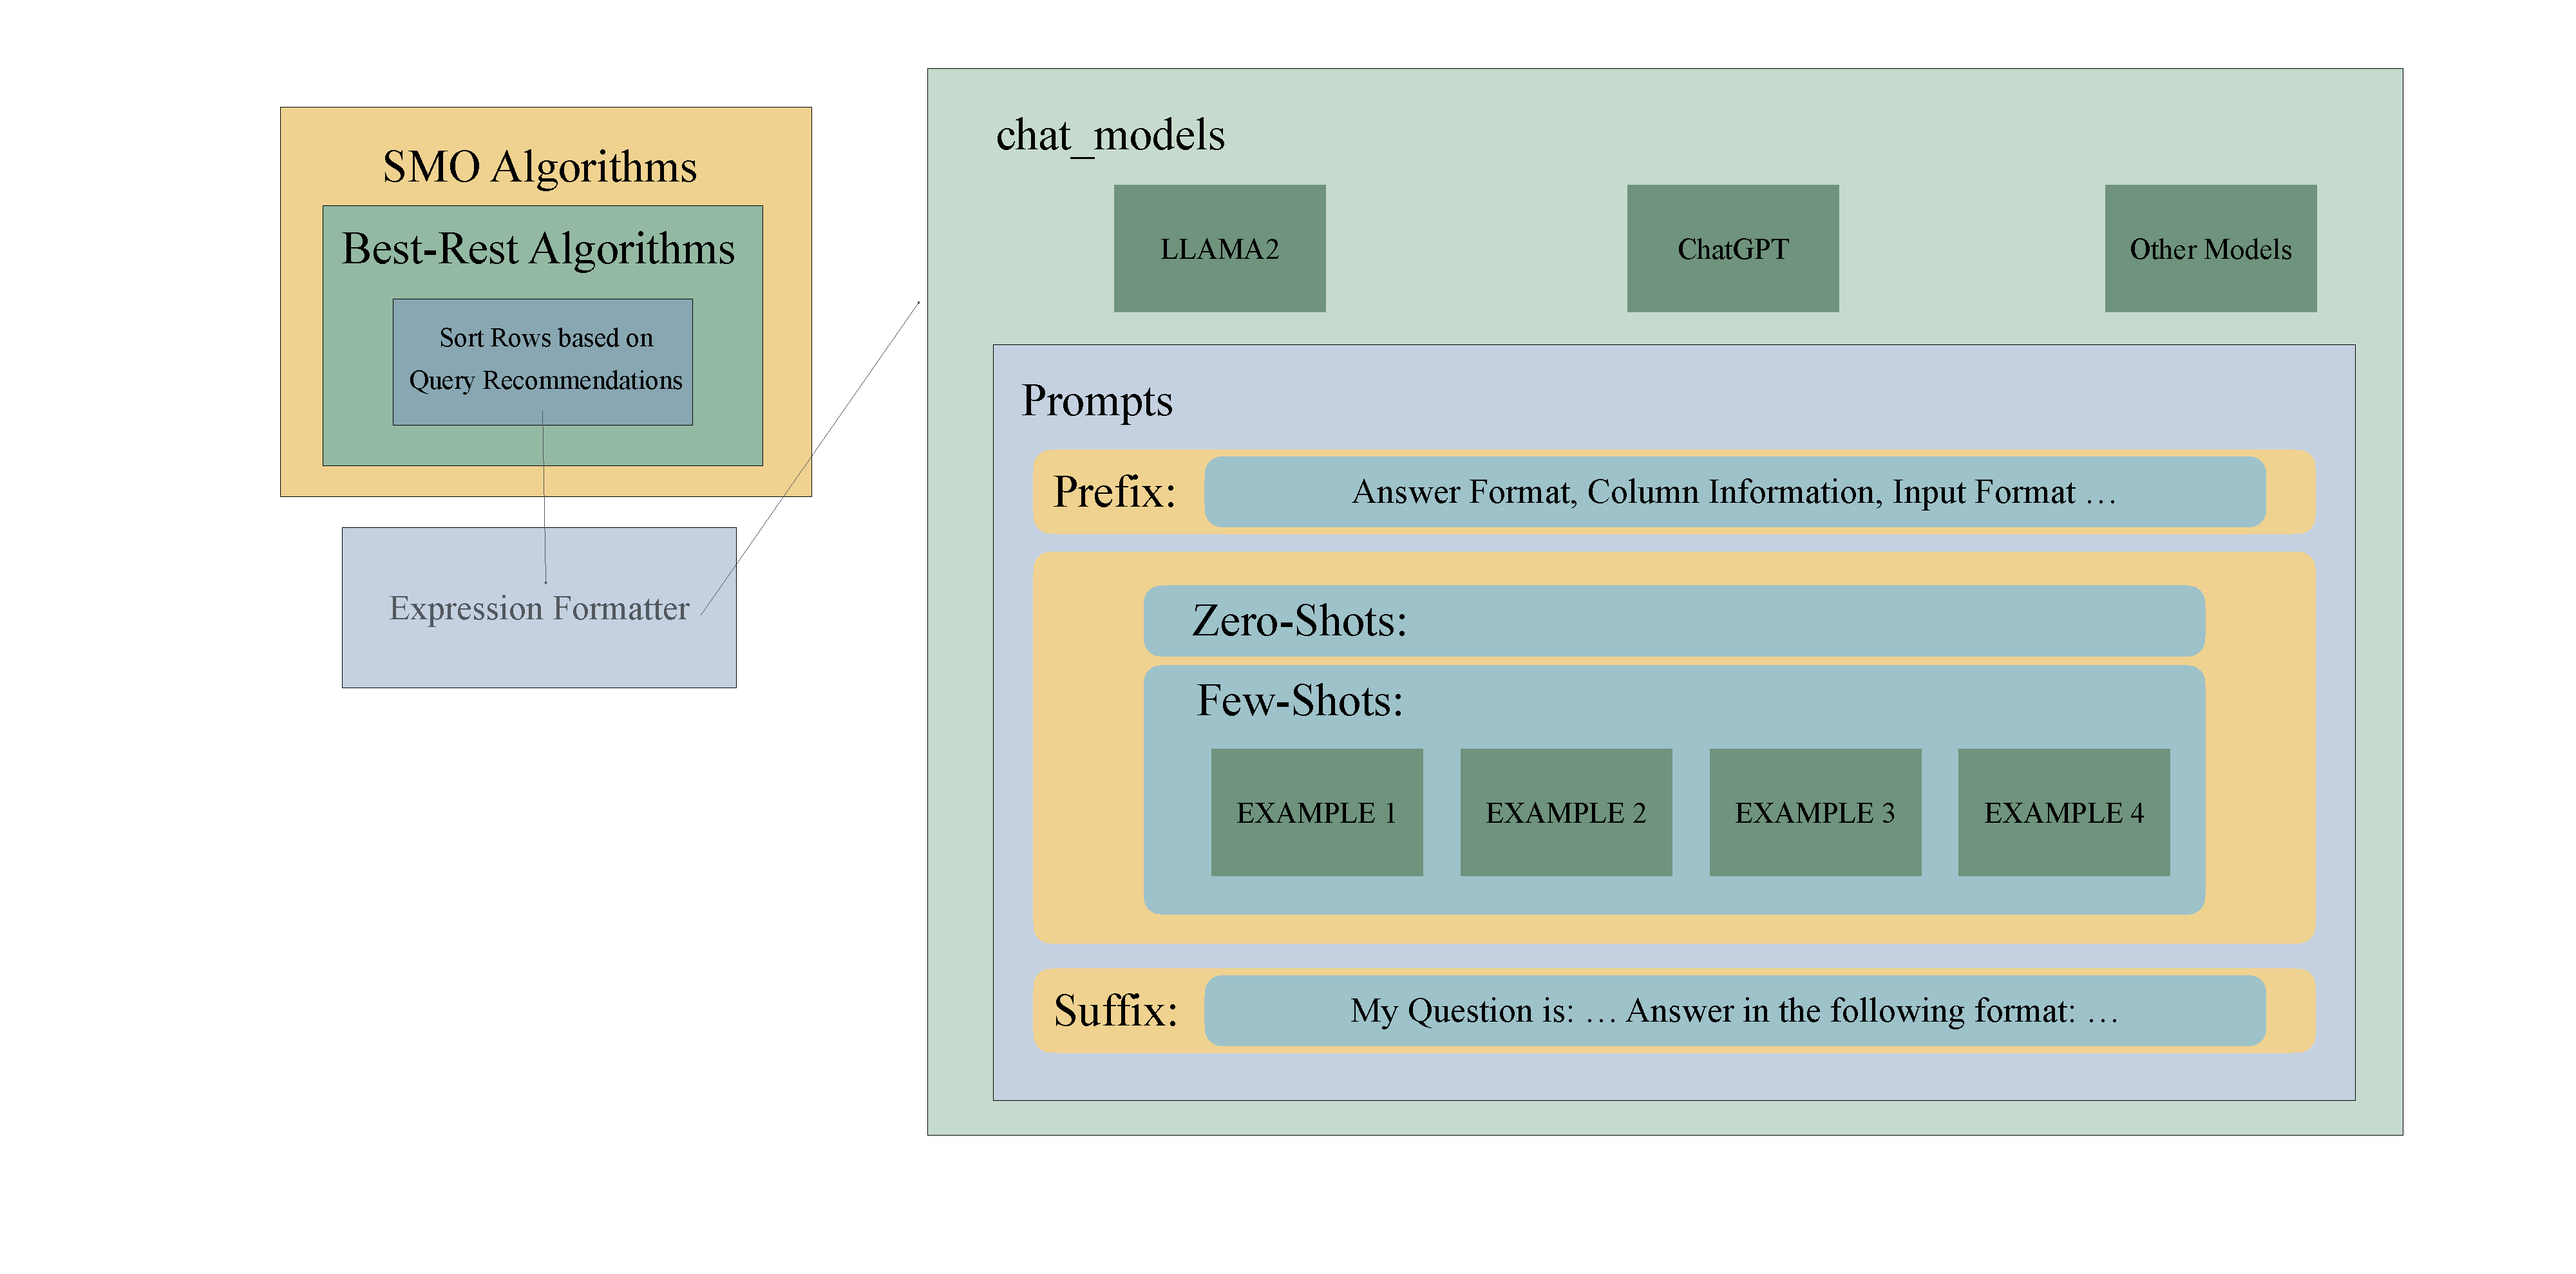
\includegraphics[page=1,width=\textwidth]{intro.pdf}
    Figure.1 An overview of ChoiceMaker \label{fig1}
  \end{figure*}

The ChoiceMaker consists of three parts, shown in Fig.\ref{fig1}: 
\begin{itemize}

\item \textbf{A modification to the SMO algorithm that sort rows based on query recommendations provided by the LLMs.}
For ease of evaluation and accuracy, we made minimal changes to the original SMO algorithm, simply replacing the original sorting algorithm with RMSE.

\item \textbf{An expression formatter}
that format the query to the LLMs specially the data rows used for sorting, and an regular expression to extract information from LLMs' outputs.

\item \textbf{A LLMs client build based on the LangChain framework.}
We introduced the LangChain library to facilitate the development of LLMs. LangChain provides an abstraction for calling APIs for different language models, and by instantiating different big predicate models, we can test different models with a unified API. The abstraction of LLMs allows us to easily switch evaluation models, such as llama2 and chatgpt. For prompts we use prefixes, examples and suffixes. In prefix, we have carefully selected the answer format, the column information and the input format for the prompt. If we want to do few-shot tunning on the model, we need to give LLMs some examples. In order to compare the performance of zero-shot with a different number of few-shots, the number of examples is optional from ${0,4,8,16}$. All examples consist of samples, and factual responses. The suffix contains the final question, usually the chosen preference, and reiterates the format of the answer to ensure that the answer can be parsed by the regular expression. In some cases of poor performance, we make artificial adjustments to the prompts, such as adding "we'll tip you" or defining the identity of the LLMs more precisely.
   
\end{itemize}

This paper makes the following contributions:
\begin{itemize}
    \item \textbf{A novel approach that empowers Sequential Model Optimization with Query Recommendations via Large Language Models(LLMs).}
    \item \textbf{Evaluation of the scalability of few shot learning}
\end{itemize}

The rest of this paper is structured as follows: Section \ref{sec:background} provides background information on the problem of choice in software engineering. Section \ref{sec:algorithms} describes the algorithms used in this work. Section \ref{sec:methods} describes the methods used in this work. Section \ref{sec:results} presents the results of the experiments. Section \ref{sec:discussion} discusses the results. Section \ref{sec:conclusion} concludes the paper.

\section{Background}
\label{sec:background}
\subsection{Sequential Model Optimization with Root Mean Square Deviation (RMSE)}
Sequential Model Optimization (SMO) is a method for optimizing the performance of a model by iteratively selecting the best model from a set of models. The RMSE is a measure of the difference between the predicted value and the actual value. The RMSE is calculated as the square root of the average of the squared differences between the predicted value and the actual value. The RMSE is a measure of the accuracy of a model, with lower values indicating better performance. The RMSE is often used as an evaluation metric in machine learning tasks, such as regression and classification. In the context of SMO, the RMSE is used to evaluate the performance of a model and select the best model from a set of models. The RMSE is calculated for each model in the set, and the model with the lowest RMSE is selected as the best model. The RMSE is used to guide the selection of models in the SMO process, with the goal of finding the model that performs best on the given task.

The RMSE formula is given by:

\begin{equation}
    \text{RMSE} = \sqrt{\frac{1}{n} \sum_{i=1}^n ( \lvert h_i - c_i \rvert)^2}
\end{equation}

where:
\begin{itemize}
    \item $n$ is the total number of observations or data points.
    \item $h_i$ represents the observed value for each data point $i$, derived from col.heaven. The "Heaven Value" (col.heaven) is a human-specific value that users can specify a \{0,1\} value to represent their preferences. For instance, if someone wants a car that's both fast and light, they could set the horsepower col.heaven to 1 and the weight col.heaven to 0 in an automotive database.
    \item $c_i$ is the calculated or expected value for each data point $i$, obtained from the expression col.norm(self.cells[col.at]). $c_i$ is a normalized value that fits within the range of 0 to 1.
    \item $(h_i - c_i)^2$ computes the square of the difference between the observed value and the calculated value for each data point.
    \item $\sqrt{\frac{1}{n} \sum_{i=1}^n (\cdot)}$ takes the square root of the average of these squared differences, yielding the RMSE, a measure of the magnitude of deviation between observed and calculated values.
\end{itemize}




\subsection{Large Language Models (LLMs)}


\section{Algorithms}
\label{sec:algorithms}

\section{Methods}
\label{sec:methods}


\section{Results}
\label{sec:results}

\section{Discussion}
\label{sec:discussion}

\section{Conclusion}
\label{sec:conclusion}



% \appendices

% Appendixes, if needed, appear before the acknowledgment.

\section*{Acknowledgment}





\begin{thebibliography}{00}



\bibitem{10352439}Long, D., Drylie, S., Ritschel, J. \& Koschnick, C. An Assessment of Rules of Thumb for Software Phase Management, and the Relationship Between Phase Effort and Schedule Success. {\em IEEE Transactions On Software Engineering}. \textbf{50}, 209-219 (2024)

\bibitem{yy} Yuanyuan Zhou, Keynote address, IEEE Automated Software Engineering conference, San Diego, California, USA, 2019. 

\bibitem{10.1145/2786805.2786852}Xu, T., Jin, L., Fan, X., Zhou, Y., Pasupathy, S. \& Talwadker, R. Hey, you have given me too many knobs!: understanding and dealing with over-designed configuration in system software. {\em Proceedings Of The 2015 10th Joint Meeting On Foundations Of Software Engineering}. pp. 307-319 (2015), https://doi.org/10.1145/2786805.2786852

\bibitem{10.1145/2961111.2962602}Han, X. \& Yu, T. An Empirical Study on Performance Bugs for Highly Configurable Software Systems. {\em Proceedings Of The 10th ACM/IEEE International Symposium On Empirical Software Engineering And Measurement}. (2016), https://doi.org/10.1145/2961111.2962602

\bibitem{9734271}Siegmund, N., Dorn, J., Weber, M., Kaltenecker, C. \& Apel, S. Green Configuration: Can Artificial Intelligence Help Reduce Energy Consumption of Configurable Software Systems?. {\em Computer}. \textbf{55}, 74-81 (2022)

\bibitem{791} Tim Menzies. Automated Software Engineering (2024 Spring) \emph{https://github.com/txt/aa24/tree/main}. 

\bibitem{b1} G. O. Young, ``Synthetic structure of industrial plastics,'' in \emph{Plastics,} 2\textsuperscript{nd} ed., vol. 3, J. Peters, Ed. New York, NY, USA: McGraw-Hill, 1964, pp. 15--64.   

\bibitem{b2} W.-K. Chen, \emph{Linear Networks and Systems.} Belmont, CA, USA: Wadsworth, 1993, pp. 123--135.

\bibitem{b3} J. U. Duncombe, ``Infrared navigation---Part I: An assessment of feasibility,'' \emph{IEEE Trans. Electron Devices}, vol. ED-11, no. 1, pp. 34--39, Jan. 1959, 10.1109/TED.2016.2628402.

\bibitem{b4} E. P. Wigner, ``Theory of traveling-wave optical laser,'' \emph{Phys. Rev}., vol. 134, pp. A635--A646, Dec. 1965.

\bibitem{b5} E. H. Miller, ``A note on reflector arrays,'' \emph{IEEE Trans. Antennas Propagat}., to be published.

\bibitem{b6} E. E. Reber, R. L. Michell, and C. J. Carter, ``Oxygen absorption in the earth's atmosphere,'' Aerospace Corp., Los Angeles, CA, USA, Tech. Rep. TR-0200 (4230-46)-3, Nov. 1988.

\bibitem{b7} J. H. Davis and J. R. Cogdell, ``Calibration program for the 16-foot antenna,'' Elect. Eng. Res. Lab., Univ. Texas, Austin, TX, USA, Tech. Memo. NGL-006-69-3, Nov. 15, 1987.

\bibitem{b8} \emph{Transmission Systems for Communications}, 3\textsuperscript{rd} ed., Western Electric Co., Winston-Salem, NC, USA, 1985, pp. 44--60.

\bibitem{b9} \emph{Motorola Semiconductor Data Manual}, Motorola Semiconductor Products Inc., Phoenix, AZ, USA, 1989.

\bibitem{b10} G. O. Young, ``Synthetic structure of industrial
plastics,'' in Plastics, vol. 3, Polymers of Hexadromicon, J. Peters,
Ed., 2\textsuperscript{nd} ed. New York, NY, USA: McGraw-Hill, 1964, pp. 15-64.
[Online]. Available:
\underline{http://www.bookref.com}.

\bibitem{b11} \emph{The Founders' Constitution}, Philip B. Kurland
and Ralph Lerner, eds., Chicago, IL, USA: Univ. Chicago Press, 1987.
[Online]. Available: \underline{http://press-pubs.uchicago.edu/founders/}

\bibitem{b12} The Terahertz Wave eBook. ZOmega Terahertz Corp., 2014.
[Online]. Available:
\underline{http://dl.z-thz.com/eBook/zomega\_ebook\_pdf\_1206\_sr.pdf}. Accessed on: May 19, 2014.

\bibitem{b13} Philip B. Kurland and Ralph Lerner, eds., \emph{The
Founders' Constitution.} Chicago, IL, USA: Univ. of Chicago Press,
1987, Accessed on: Feb. 28, 2010, [Online] Available:
\underline{http://press-pubs.uchicago.edu/founders/}

\bibitem{b14} J. S. Turner, ``New directions in communications,'' \emph{IEEE J. Sel. Areas Commun}., vol. 13, no. 1, pp. 11-23, Jan. 1995.

\bibitem{b15} W. P. Risk, G. S. Kino, and H. J. Shaw, ``Fiber-optic frequency shifter using a surface acoustic wave incident at an oblique angle,'' \emph{Opt. Lett.}, vol. 11, no. 2, pp. 115--117, Feb. 1986.

\bibitem{b16} P. Kopyt \emph{et al., ``}Electric properties of graphene-based conductive layers from DC up to terahertz range,'' \emph{IEEE THz Sci. Technol.,} to be published. DOI: 10.1109/TTHZ.2016.2544142.

\bibitem{b17} PROCESS Corporation, Boston, MA, USA. Intranets:
Internet technologies deployed behind the firewall for corporate
productivity. Presented at INET96 Annual Meeting. [Online].
Available: \underline{http://home.process.com/Intranets/wp2.htp}

\bibitem{b18} R. J. Hijmans and J. van Etten, ``Raster: Geographic analysis and modeling with raster data,'' R Package Version 2.0-12, Jan. 12, 2012. [Online]. Available: \underline {http://CRAN.R-project.org/package=raster} 

\bibitem{b19} Teralyzer. Lytera UG, Kirchhain, Germany [Online].
Available:
\underline{http://www.lytera.de/Terahertz\_THz\_Spectroscopy.php?id=home}, Accessed on: Jun. 5, 2014

\bibitem{b20} U.S. House. 102\textsuperscript{nd} Congress, 1\textsuperscript{st} Session. (1991, Jan. 11). \emph{H. Con. Res. 1, Sense of the Congress on Approval of}  \emph{Military Action}. [Online]. Available: LEXIS Library: GENFED File: BILLS

\bibitem{b21} Musical toothbrush with mirror, by L.M.R. Brooks. (1992, May 19). Patent D 326 189 [Online]. Available: NEXIS Library: LEXPAT File: DES

\bibitem{b22} D. B. Payne and J. R. Stern, ``Wavelength-switched pas- sively coupled single-mode optical network,'' in \emph{Proc. IOOC-ECOC,} Boston, MA, USA, 1985, pp. 585--590.

\bibitem{b23} D. Ebehard and E. Voges, ``Digital single sideband detection for interferometric sensors,'' presented at the \emph{2\textsuperscript{nd} Int. Conf. Optical Fiber Sensors,} Stuttgart, Germany, Jan. 2-5, 1984.

\bibitem{b24} G. Brandli and M. Dick, ``Alternating current fed power supply,'' U.S. Patent 4 084 217, Nov. 4, 1978.

\bibitem{b25} J. O. Williams, ``Narrow-band analyzer,'' Ph.D. dissertation, Dept. Elect. Eng., Harvard Univ., Cambridge, MA, USA, 1993.

\bibitem{b26} N. Kawasaki, ``Parametric study of thermal and chemical nonequilibrium nozzle flow,'' M.S. thesis, Dept. Electron. Eng., Osaka Univ., Osaka, Japan, 1993.

\bibitem{b27} A. Harrison, private communication, May 1995.

\bibitem{b28} B. Smith, ``An approach to graphs of linear forms,'' unpublished.

\bibitem{b29} A. Brahms, ``Representation error for real numbers in binary computer arithmetic,'' IEEE Computer Group Repository, Paper R-67-85.

\bibitem{b30} IEEE Criteria for Class IE Electric Systems, IEEE Standard 308, 1969.

\bibitem{b31} Letter Symbols for Quantities, ANSI Standard Y10.5-1968.

\bibitem{b32} R. Fardel, M. Nagel, F. Nuesch, T. Lippert, and A. Wokaun, ``Fabrication of organic light emitting diode pixels by laser-assisted forward transfer,'' \emph{Appl. Phys. Lett.}, vol. 91, no. 6, Aug. 2007, Art. no. 061103.~

\bibitem{b33} J. Zhang and N. Tansu, ``Optical gain and laser characteristics of InGaN quantum wells on ternary InGaN substrates,'' \emph{IEEE Photon. J.}, vol. 5, no. 2, Apr. 2013, Art. no. 2600111

\bibitem{b34} S. Azodolmolky~\emph{et al.}, Experimental demonstration of an impairment aware network planning and operation tool for transparent/translucent optical networks,''~\emph{J. Lightw. Technol.}, vol. 29, no. 4, pp. 439--448, Sep. 2011.

\end{thebibliography}

% \begin{IEEEbiography}[{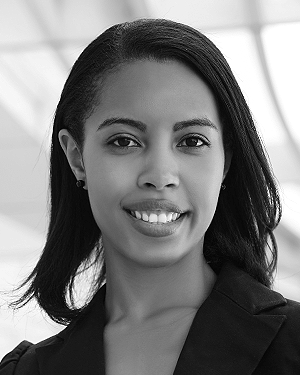
\includegraphics[width=1in,height=1.25in,clip,keepaspectratio]{a1.png}}]{First A. Author} (M'76--SM'81--F'87) and all authors may include 
% biographies. Biographies are often not included in conference-related
% papers. This author became a Member (M) of IEEE in 1976, a Senior
% Member (SM) in 1981, and a Fellow (F) in 1987. The first paragraph may
% contain a place and/or date of birth (list place, then date). Next,
% the author's educational background is listed. The degrees should be
% listed with type of degree in what field, which institution, city,
% state, and country, and year the degree was earned. The author's major
% field of study should be lower-cased. 

% The second paragraph uses the pronoun of the person (he or she) and not the 
% author's last name. It lists military and work experience, including summer 
% and fellowship jobs. Job titles are capitalized. The current job must have a 
% location; previous positions may be listed 
% without one. Information concerning previous publications may be included. 
% Try not to list more than three books or published articles. The format for 
% listing publishers of a book within the biography is: title of book 
% (publisher name, year) similar to a reference. Current and previous research 
% interests end the paragraph. The third paragraph begins with the author's 
% title and last name (e.g., Dr.\ Smith, Prof.\ Jones, Mr.\ Kajor, Ms.\ Hunter). 
% List any memberships in professional societies other than the IEEE. Finally, 
% list any awards and work for IEEE committees and publications. If a 
% photograph is provided, it should be of good quality, and 
% professional-looking. Following are two examples of an author's biography.
% \end{IEEEbiography}

% \begin{IEEEbiography}[{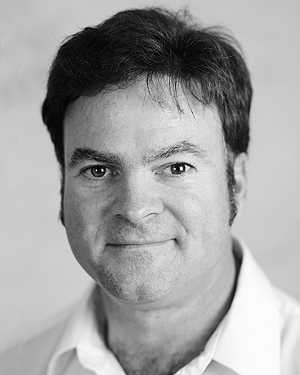
\includegraphics[width=1in,height=1.25in,clip,keepaspectratio]{a2.png}}]{Second B. Author} was born in Greenwich Village, New York, NY, USA in 
% 1977. He received the B.S. and M.S. degrees in aerospace engineering from 
% the University of Virginia, Charlottesville, in 2001 and the Ph.D. degree in 
% mechanical engineering from Drexel University, Philadelphia, PA, in 2008.

% From 2001 to 2004, he was a Research Assistant with the Princeton Plasma 
% Physics Laboratory. Since 2009, he has been an Assistant Professor with the 
% Mechanical Engineering Department, Texas A{\&}M University, College Station. 
% He is the author of three books, more than 150 articles, and more than 70 
% inventions. His research interests include high-pressure and high-density 
% nonthermal plasma discharge processes and applications, microscale plasma 
% discharges, discharges in liquids, spectroscopic diagnostics, plasma 
% propulsion, and innovation plasma applications. He is an Associate Editor of 
% the journal \emph{Earth, Moon, Planets}, and holds two patents. 

% Dr. Author was a recipient of the International Association of Geomagnetism 
% and Aeronomy Young Scientist Award for Excellence in 2008, and the IEEE 
% Electromagnetic Compatibility Society Best Symposium Paper Award in 2011. 
% \end{IEEEbiography}

% \begin{IEEEbiography}[{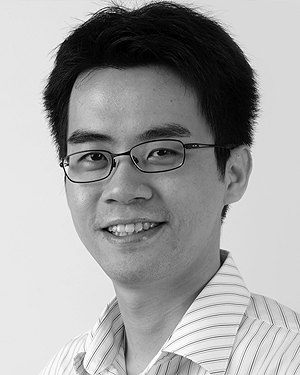
\includegraphics[width=1in,height=1.25in,clip,keepaspectratio]{a3.png}}]{Third C. Author, Jr.} (M'87) received the B.S. degree in mechanical 
% engineering from National Chung Cheng University, Chiayi, Taiwan, in 2004 
% and the M.S. degree in mechanical engineering from National Tsing Hua 
% University, Hsinchu, Taiwan, in 2006. He is currently pursuing the Ph.D. 
% degree in mechanical engineering at Texas A{\&}M University, College 
% Station, TX, USA.

% From 2008 to 2009, he was a Research Assistant with the Institute of 
% Physics, Academia Sinica, Tapei, Taiwan. His research interest includes the 
% development of surface processing and biological/medical treatment 
% techniques using nonthermal atmospheric pressure plasmas, fundamental study 
% of plasma sources, and fabrication of micro- or nanostructured surfaces. 

% Mr. Author's awards and honors include the Frew Fellowship (Australian 
% Academy of Science), the I. I. Rabi Prize (APS), the European Frequency and 
% Time Forum Award, the Carl Zeiss Research Award, the William F. Meggers 
% Award and the Adolph Lomb Medal (OSA).
% \end{IEEEbiography}

\EOD

\end{document}
